\section{Introduction}

\section{Related Work}
The first part of this chapter provides an overview of the related work in the field of
Information Visualization. First general methods, which are important for visualizations of heterogeneous data in this area of application, are described. This rather high level discussion is followed by a more specialized view on map-based visualizations and transitions in visualizations. The combination of these two emerging research areas leads to the application of map-based visualizations with transitions between them. Finally the current state in the domain of map-based visualization is summarized and potential improvements are identified.

\subsection{GeoVisualization methods}
 Thus visualization now also emphasizes the knowledge creation and hypothesis generation aspects of \ac{SciVis}.

In the early 1980s, a french graphic theorist named Jacques Bertin set a milestone in the area of scientific research. Based on his work in this \ac{GeoVis} developed as a field of research. His work shows a strong focus in the research of the potential for the use of dynamic visual displays as prompts for scientific insight and of the methods through which dynamic visual displays might leverage perceptual cognitive processes to facilitate scientific thinking \iacite{maceachren:2004}.

As already mentioned, \ac{GeoVis} is closely related to the fields of \ac{SciVis} and also \ac{InfoVis} and emphasizes knowledge construction over knowledge storage or information transmission \iacite{maceachren:1997}. However \ac{InfoVis} needs to be strictly differentiated from \ac{SciVis}. \ac{InfoVis} deals with abstract data like for example movies in a movie database whereas \ac{SciVis} operates on real-world data with spatial character.

\ac{GeoVis} also contributes significantly to other related fields such as \ac{SciVis} and also \ac{InfoVis}. Owing to its roots in cartography, \ac{GeoVis} contributes to these other fields by way of the map metaphor, which "[\ldots] has been widely used to visualize non-geographic information in the domains of information visualization and domain knowledge visualization" \iacite{Jiang2005}. It emphasizes knowledge construction over knowledge storage or information transmission \iacite{maceachren:1997}. However \ac{InfoVis} needs to be strictly differentiated from \ac{SciVis}. \ac{InfoVis} deals with abstract data like for example movies in a movie database whereas \ac{SciVis} operates on real-world data with spatial character.

Traditional, static maps have a limited exploratory capability. The graphical representations are inextricably linked to the geographical information beneath. \ac{GIS} and \ac{GeoVis} allow for more interactive maps. Both of them have the ability to extend the basic layer of a map with user-experience abilities like for example zooming in or out and to change the visual appearance of the map \iacite{Jiang2003}.

This kind of visualization is also used in practical applications. The following list shows some summarized examples of those:
\begin{description}

\item[Urban Planning] \hfill \\
Urbanists use \ac{GeoVis} to "[\ldots] model environmental interests and policy concerns of the general public" \iacite{Jiang2003}. \citeauthor{Jiang2003} also mention two examples, in which "[\ldots] 3D photorealistic representations are used to show urban redevelopment and dynamic computer simulations are used to show possible pollution diffusion over the next few years".

\citeauthor{Jiang2003} also describe that the widespread use of the internet by the general public allows collaborative planning to be conducted in both centralised and decentralised manner. The former way of planning in committee rooms or computer facility rooms can be extended with a decentralised web platform. This platform would lead to increased parcitipation by the public because
\begin{enumerate}
\item the internet already integrates various interactive and proactive techniques and
\item is time and place independent.
\end{enumerate}

\item[Environmental Studies] \hfill \\
\citeauthor{Danado2005} describe a system that is capable of simulating and visualizing environmental processes with the ability to retrieve additional information while moving through the environmental area in real time. Each user of the system is able to impact the simulation by adding or removing so called agents to or from the model. Those agents will affect the environment with the decisions the users made. Users therefore can use this system to explore a complex set of environmental data, interrogate a number of scenarios or policy options to determine a best fit \iacite{Danado2005}.

\item[Forestry] \hfill \\
\citeauthor{Andrienko2007} present a system to visualize a large set of spatio-temporal data related to european forests. The innovative approach of this system is given by allowing the data to be explored interactively by non-experts over the internet. Furthermore \citeauthor{Andrienko2007} state their approach "[\ldots] uncovers a range of fundamental issues relevant to the broad field of \ac{GeoVis} and \ac{InfoVis} research."

\citeauthor{Andrienko2007} also cited the two major problems as
\begin{enumerate}
\item the inability of the geovisualizers to convince the foresters of the efficiency of \ac{GeoVis} in their work and
\item the foresters' misgivings over the dataset's accessibility to non-experts engaging in "uncontrolled exploration".
\end{enumerate}

\item[Telecommunication] \hfill \\
\ac{GeoVis} are also very helpful in the area of telecommunication. Telegeography\footnote{https://www.telegeography.com/}, as an example for a company in that specific area, has an interactive submarine cable map. Figure \ref{fig:submarine} and \ref{fig:submarine-interactive} are showing this map and its interactivity which gives more information to the cable’s profile, including the cable’s name, ready-for-service date, length, owners, website, and landing points.

\begin{figure}[h]
\centering
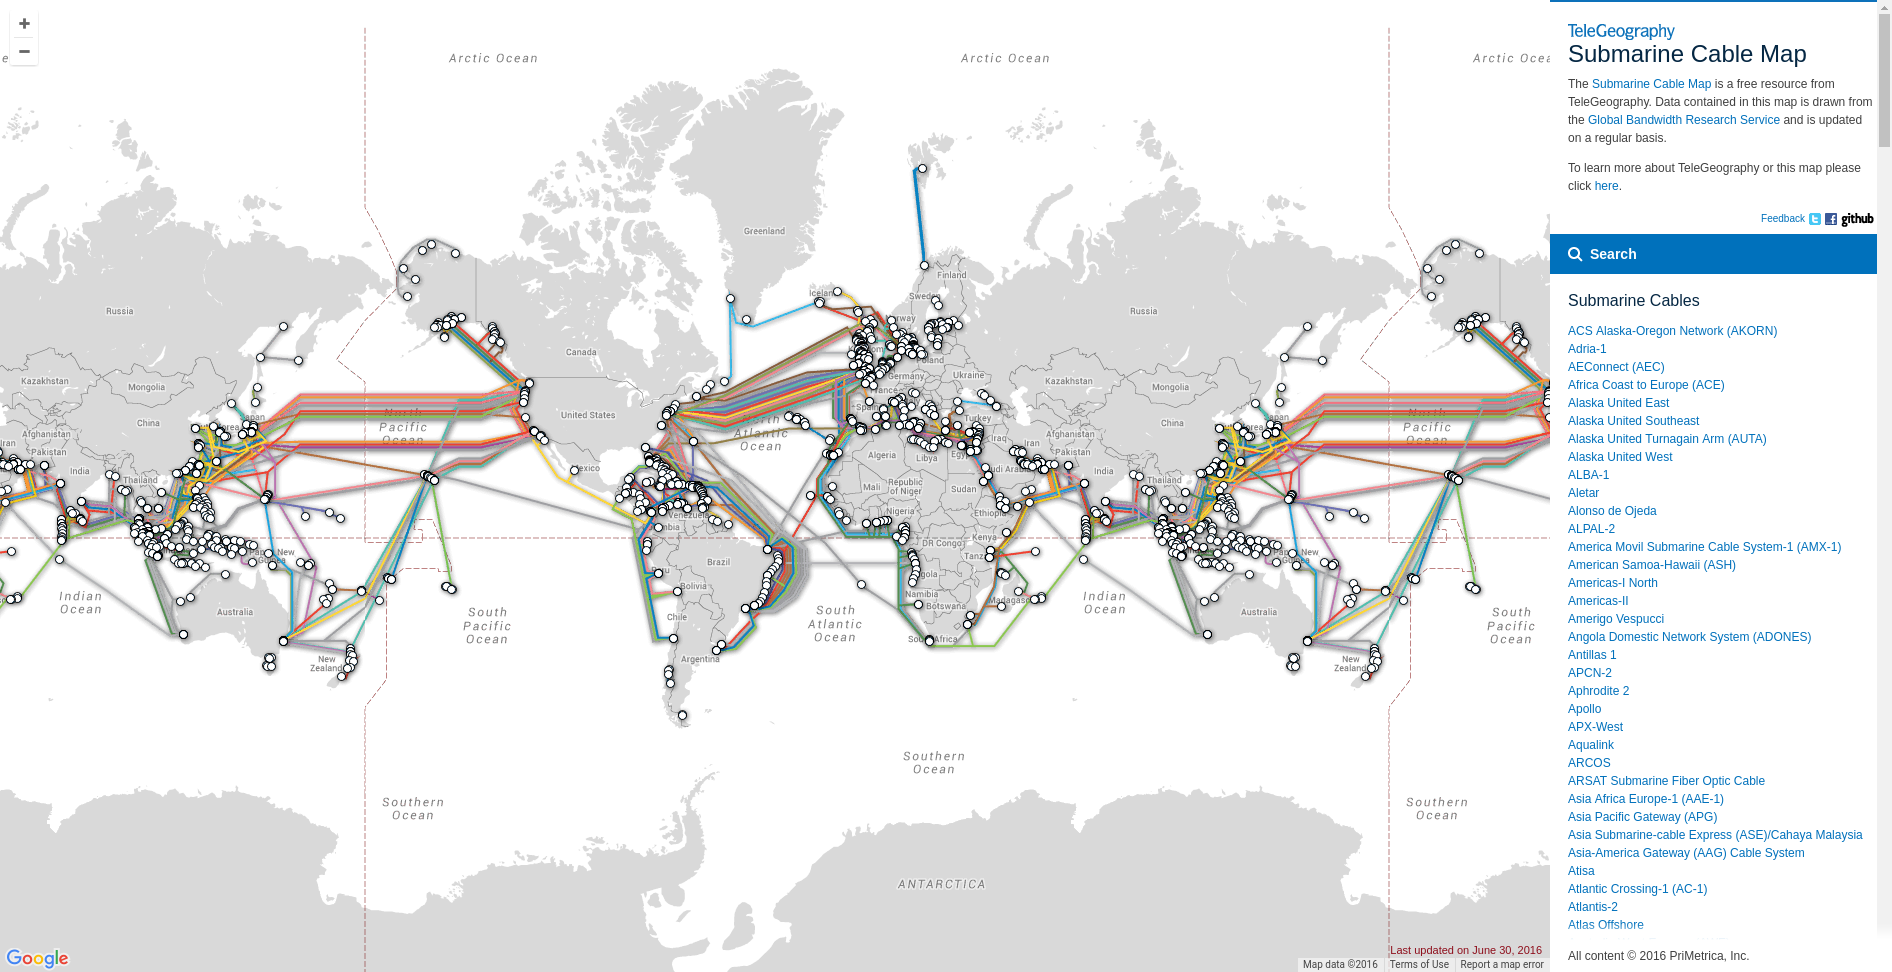
\includegraphics[width=0.8\textwidth,keepaspectratio]{images/geovis/submarine.png}
\caption[
    TeleGeography’s free interactive submarine cable map, Urldate: 07.2016 \newline
\small\texttt{\url{http://www.submarinecablemap.com/}}
]{TeleGeography’s free interactive submarine cable map}
\label{fig:submarine}
\end{figure}

\begin{figure}[h]
\centering
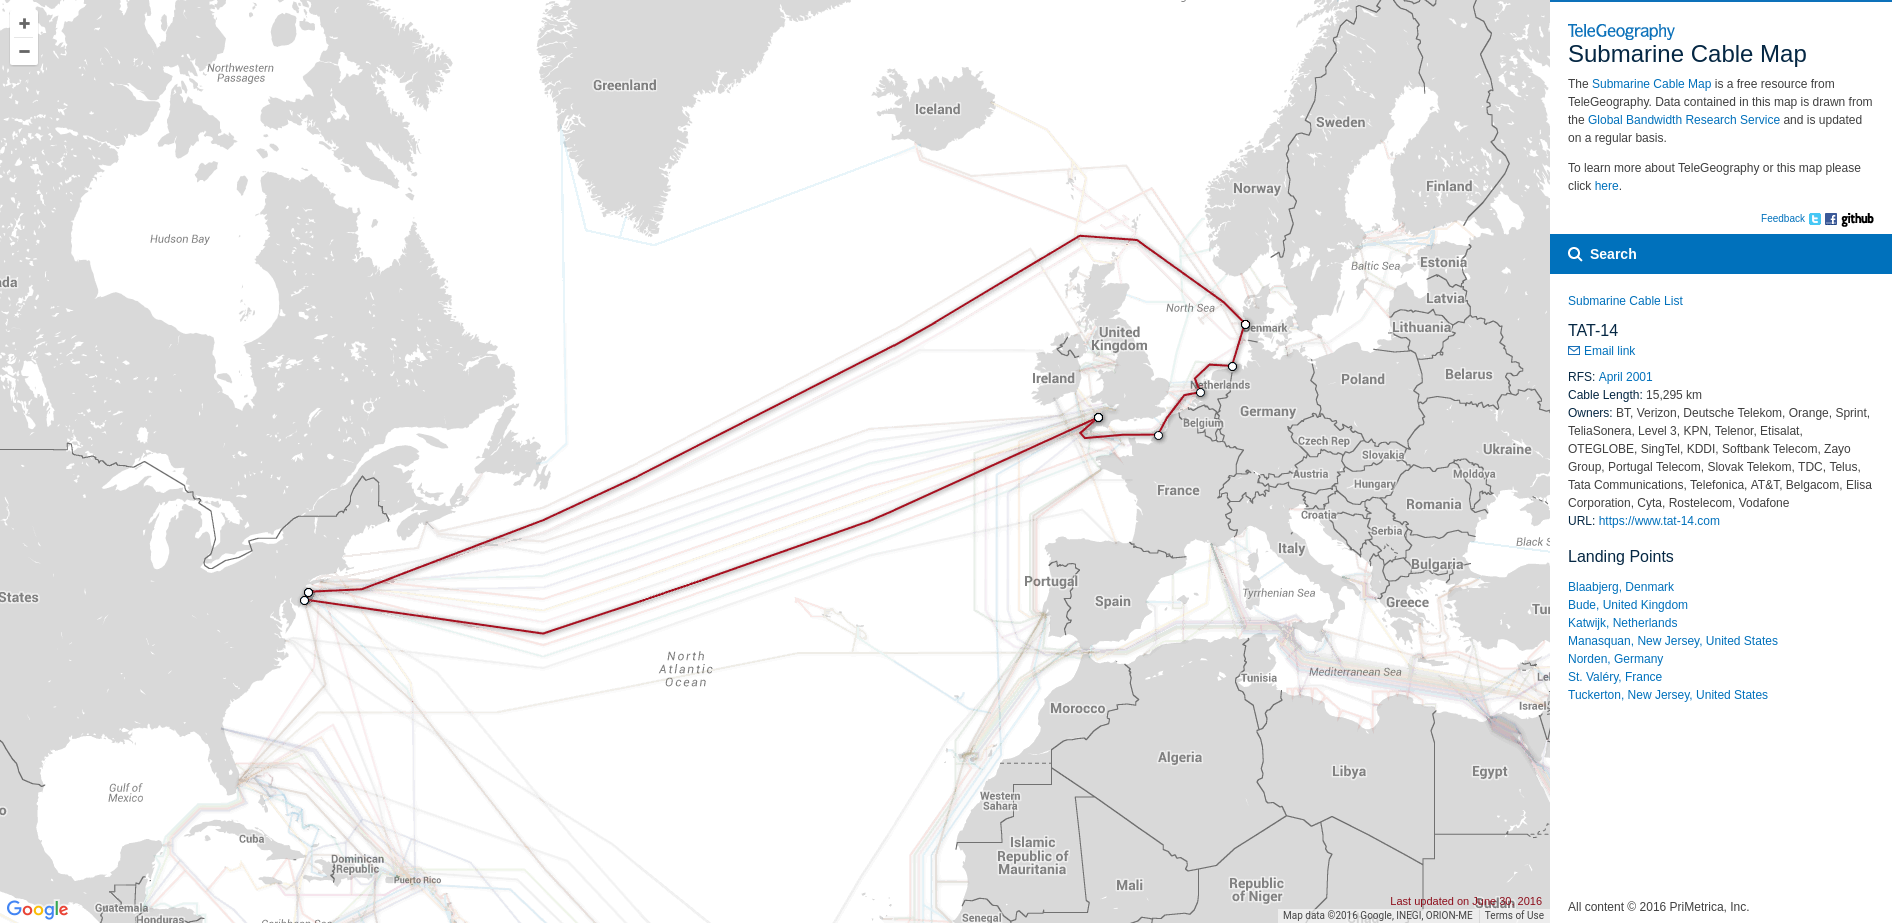
\includegraphics[width=0.8\textwidth,keepaspectratio]{images/geovis/submarine-interactive.png}
\caption[
    TeleGeography’s free interactive submarine cable map, Urldate: 07.2016 \newline
\small\texttt{\url{http://www.submarinecablemap.com/}}
]{TeleGeography’s free interactive submarine cable map}
\label{fig:submarine-interactive}
\end{figure}

\item[E-commerce] \hfill \\
\ac{GeoVis} can be very useful in analysing data provided by e-commerce shops if they track online orders with some kind of geographical information. If such data is available and provided, it is possible to easily visualize the target group of a company on a map and therefore  create knowledge and allow for generating hypothesis i.e. the next region for expansion.

\end{description}